\documentclass{labReport}
\urlstyle{same}

\let\verbatim\undefined 
\let\verbatimend\undefined 
\lstnewenvironment{verbatim}{\lstset{breaklines,basicstyle=\ttfamily}}{}
\usepackage{lipsum}
\usepackage{graphicx}
\usepackage{float}


\title{Lab 4: Divide and Conquer Algorithms}
\author{Adam Haile, Aiden Miller, Leigh Goetsch}
\prof{Dr. Berisha}
\className{Algorithms \& Adv. Data Struct.}
\classCode{CSC 3310}
\semester{Fall 2024}
\submissionDate{11/08/2024}
\labWeek{8}
\laboratoryDate{10/25/2024}

\begin{document}
\maketitle

\section*{Learning Outcomes}
\begin{itemize}
    \item Read and interpret a written description of an algorithm
    \item Correctly implement an algorithm from pseudocode
    \item Generate test cases for the implementation
    \item Design and execute benchmarks for an algorithm
    \item Repo: \url{https://github.com/jeffTheLandShark/CSC3310/tree/main/Lab5}
\end{itemize}

% if you want a TOC:
% \tableofcontents

\newpage
% if you want to use multicols:
% \begin{multicols*}{2}
% \raggedcolumns

\section{Paper Review}
\begin{enumerate}
    \item How do scapegoat trees compare with Red-Black, AVL, and splay trees? Why might you prefer to use or not use a scapegoat tree?\\
    Scapegoat trees do not maintain a strict balance of the binary tree, instead they will allow imbalances up to a certain threshold $\alpha$. This results in an insertion and deletion of amortized $O(log n)$. They also do not maintain additional information like splay trees. They are generally easier to implement than AVL or Red-Black trees due to not needing a strict ruleset for balancing and complex rotations. The issue is that they can have an expensive worst-case of $O(n)$, and are not quite as adaptive to access patterns. 
    \item What does it mean for a node to be weight balanced? What does it mean for a tree to be weight-balanced? Draw some examples and calculate their weight balances.\\
    A node in a tree is weight-balanced if the sizes of its left and right subtrees are proportional according to the parameter $\alpha$. A tree is weight-balanced if all its nodes satisfy the weight balance condition for the chosen $\alpha$. This ensures that no subtree is disproportionately large compared to its sibling, indirectly controlling the height of the tree. \\
    Example: \\
    Balanced Tree ($\alpha = 0.75$) \\
    \begin{verbatim}
        1
       / \
      2   3
     / \
    4   5
    \end{verbatim}
    Unbalanced Tree ($\alpha = 0.75$)
    \begin{verbatim}
        10
       /  \
      5    20
     / \
    2   7
         \
          8 
    \end{verbatim}
    \item What is the interpretation of the $\alpha$ parameter?\\
    The $\alpha$ parameter is a balancing threshold that determines how evently distributed the sizes of the subtrees of a node must be to maintain a balanced tree structure. $\alpha$ defines a maximum proportion of the total size of a node's subtree that any single child subtree can have.
    \item What are the conditions for triggering a rebuild of a subtree (during inserts) or the entire tree (during deletes)?\\
    The conditions for trigger a rebuild of a subtree or the entire tree depend on the violation of the $\alpha$ parameter. For subtree rebuild during inserts, if: \\
    \[
    \text{size(left[x])} > \alpha \cdot \text{size(x)} \text{ or } \text{size(right[x])} > \alpha \cdot \text{size(x)}
    \]
    Where size(x) is the size of the subtree rooted at x. \\
    For tree rebuild during deletes, if: \\
    \[
    \text{size(T)} < \alpha \cdot \text{max-size(T)}
    \]
    Where size(T) is the current number of nodes in the tree and max-size(T) is the largest size the tree has had since its last rebuild.

\end{enumerate}

\section{Implementation}

% Implement a scapegoat tree that supports insert, size, delete, and contains operations. The treeshould additionally support a toList() operation that generates a list from an in-order traversal. Add a counter variable to keep track of the number of times the rebuild operation is performed. You do not need to implement the logarithmic space rebuild algorithm described in 6.1 and 6.2 - use the straightforward approach.

% Write unit tests that involve the insert, remove, size, contains, and toList() operations.
\begin{table}[h!]
    \centering
    \begin{tabular}{|c|c|c|}
    \hline
    Test & Description & Result \\
    \hline
    Test 1 & Test empty tree & Pass \\
    Test 2 & Test single node insertion & Pass \\
    Test 3 & Test balanced tree & Pass \\
    Test 4 & Test multiple insertions & Pass \\
    Test 5 & Test deletion & Pass \\
    Test 6 & Test toList() & Pass \\
    Test 7 & Test reverse order list & Pass \\
    Test 8 & Test in order list insert with empty list & Pass \\
    \hline
    \end{tabular}
    \caption{Test Results}
    \label{table:test_results}
\end{table}

\subsection{Benchmarking}
% Benchmark the insert, delete, and contains operations of your implementation on data sets of different sizes. Create tables and plots that include both run times and the number of times the rebuild operation was performed.

\begin{figure}[H]
    \centering
    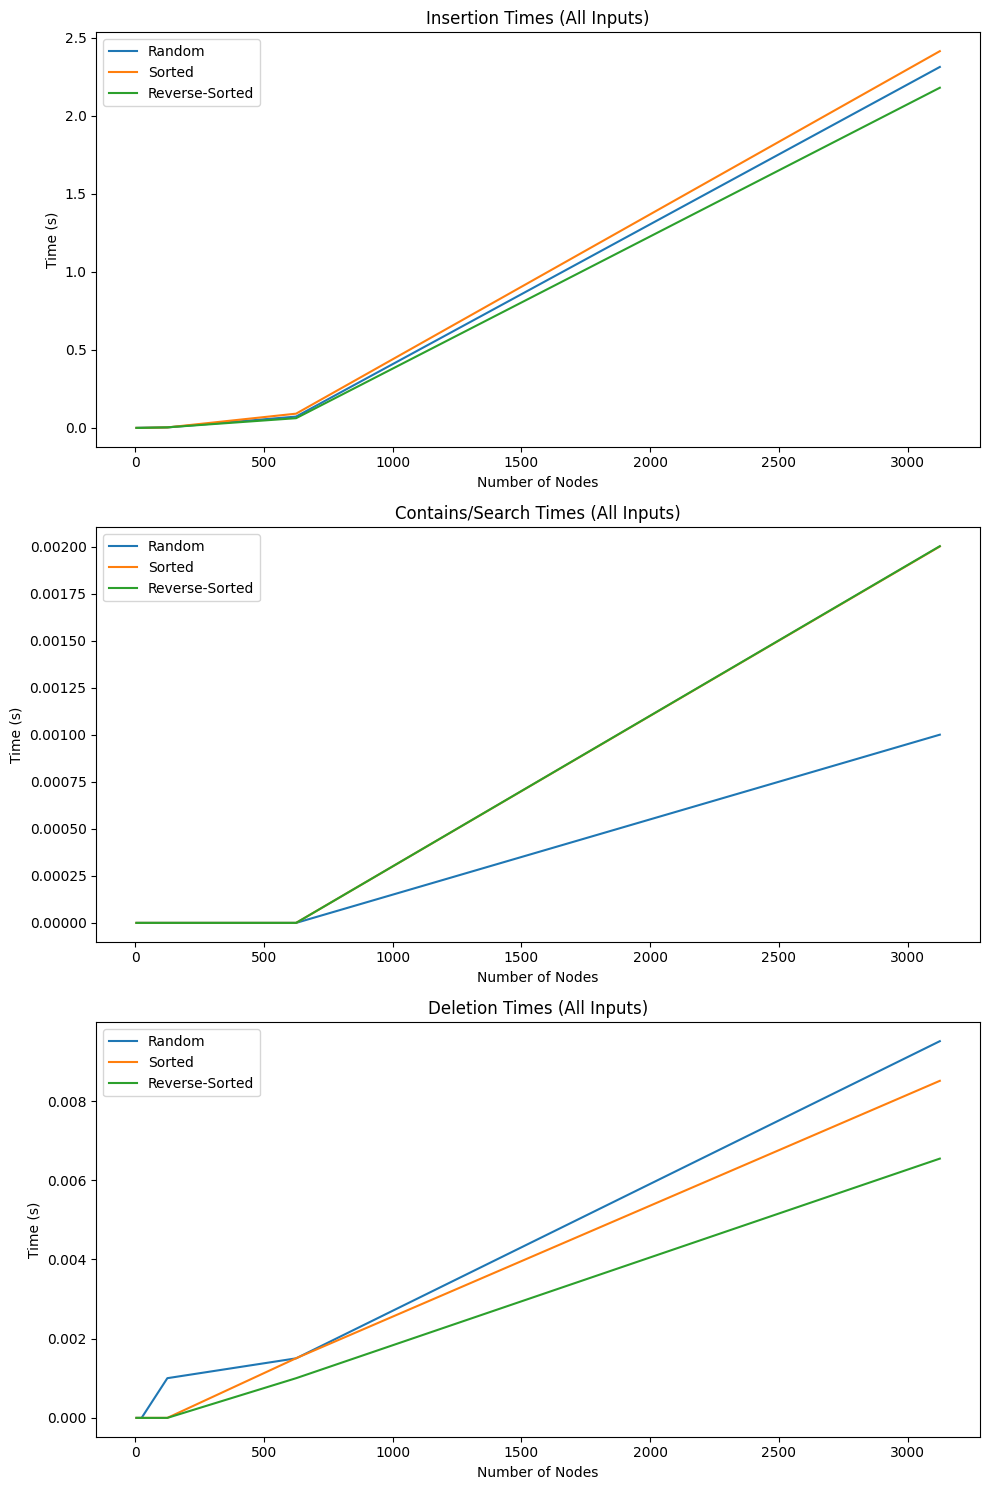
\includegraphics[width=0.8\textwidth]{benchmarks.png}
    \caption{Benchmark results for Scapegoat Tree operations}
    \label{fig:benchmark}
\end{figure}

\subsection{Benchmarking Analysis}
% Analyze and interpret the benchmark results to determine if the run time of your implementation is consistent with the theoretical analysis.
The benchmark results for the scapegoat tree operations are shown in Figure~\ref{fig:benchmark}. These results include the runtime for `insert`, `delete`, and `contains` operations on datasets of varying sizes, as well as the frequency of rebuild operations. We do generally see consistent trends that we would expect of an $O(log \: n)$ runtime for insertion, contains, and deletion, with some fringing on an $O(n)$ runtime which we can expect as a worst-case for any of these depending on the values being input and the amount of times the tree needs to be rebalanced.

% \end{multicols*}

% add appendix
% 7. Attach all your source code and test cases in an appendix.



\end{document}
